\chapter{Marco Teórico} 
\label{sec:marcoteorico}

Este capitulo tiene como objeto introducir los conocimiento sobre sistemas de posicionamiento Global (GPS) y los aspectos técnicos relacionados con la señales y su recepción en dispositivos de posicionamiento (receptores).

\section{Sistema global de posicionamiento satelital - GNSS}

El sistema de posicionamiento global (GPS), es el primer sistema global de navegación satelital GNSS. GPS consta de una constelación de 24 satélites sobre la orbital media de la tierra que trasmite continuamente señales de radio frecuencia hacia la tierra, permitiendo así que los dispositivos de posicionamiento puedan determinar su posición sobre la superficie terrestre.\\

La idea detrás de los sistemas de posicionamiento tales como GPS, puede resumirse en que:\\

\textit{Si la distancia desde tres satélites en el espacio a un punto en común sobre la superficie de la tierra(un receptor GPS) es conocida, junto con la posición de los satélites al momento de la transmisión, la posición del receptor puede ser determinada gracias a la aplicación de conceptos trigonométricos, álgebra y un sistema de coordenadas apropiado.\cite{Thompson_1998}.}\\

Sin embargo, la problemática es ¿Como conseguir las distancias a cada satélite de forma precisa, para poder aumentar la precisión al momento de determinar la posición del receptor sobre la superficie de la tierra.?\\

Para ello es necesario profundizar mas los conceptos y conocimientos acerca del funcionamiento de GPS.

\subsection{El funcionamiento GPS}

GPS funciona gracias a la transmisión continua de señales de radiofrecuencia a través de la ionosfera y la troposfera. Las señales transmitidas están conformadas por dos señales de portadora, dos códigos y un mensaje de navegación (detalles acerca del satélite). Estas señales son adquiridas gracias una antena especialmente diseñada para captar la señales en el rango de frecuencias específicos en que transmiten los satélites GPS (1227.60 y 1575.42 MHz).\\

Posterior a la adquisición y decodificación de la señal viene una etapa de cálculos en la que un componente de software realiza cálculos para descifrar que mensaje de navegación corresponde a determinado satélite, gracias a los códigos recibidos de manera simultanea.\\


%\subsubsection
\textbf{Triangulación y trilateración.}\\

Triangulación es el método o forma más común para la  determinación de una posición sobre la superficie terrestre basada en puntos de referencias o “faros”. Para ello, los ángulos entre el receptor y los puntos de referencia deben ser conocidos para que receptor puede determinar su posición; en este escenario, la precisión con la que el receptor determina su posición, depende de la precisión con la que puede medir los ángulos con respecto a cada punto de referencia.\\
 
La Trilateración, es un método apoyado en el conocimiento de las posiciones de los puntos de referencia. En este caso, la precisión con la que el receptor puede determinar su posición depende estrictamente de la exactitud con la que puede medir la distancia hasta el punto de referencia. En este concepto se apoya el funcionamiento de GPS.

\section{Modelos observacionales y técnicas de posicionamiento}

Los observables de medición arrojado por los dispositivos de posicionamiento son el resultado de los procedimientos internos del receptor para la estimación de los tiempos de viaje de la señal, luego de las etapas de adquisición y de-modulación. Los observables entregados por los dispositivos GPS, pueden estar expresados en formato propietario(binario) o acogidos a estándares como \textbf{NMEA\footnote{NMEA: National Marine Electronics Association,  http://www.gpsinformation.org/dale/nmea.htm}} y \textbf{RINEX\footnote{RINEX: Receiver INdependent EXchange, https://igscb.jpl.nasa.gov/igscb/data/format/rinex211.txt}}.\\

%\subsection{Representación numérica de las señales}

En teoría, una vez las señales han sido decodificadas y clasificadas, con el conocimiento de las distancias de tres satélites hasta el punto donde se ubica el receptor, es posible mediante la solución a un sistema de ecuaciones que tiene como incógnitas las coordenadas X, Y, Z donde se encuentra el receptor. Sin embargo, un cuarto satélite es necesario para una cuarta variable (tiempo), la cual hace referencia al momento exacto en el que el receptor recibir las señales que le permiten posicionarse.\\

Dado que las fuentes de error a las que está expuesta la señal que viaja entre el satélite y el receptor pueden afectar la fidelidad del observable, se emplean modelos matemáticos para representar el valor medido (observable), como una expresión que contiene el valor real a medir (distancia) y la ponderación de las fuentes de error que contaminan la medición.

\subsection{Posicionamiento Autónomo %(Single Point Positioning Model)
}

Es quizás el método de posicionamiento más sencillo y autónomo que puede permitir localizar un receptor sobre la superficie de la tierra. Este método es la base inicial para llevar a cabo tareas de posicionamiento mediante GPS. El modelo SPP como comúnmente se le conoce, plantea la introducción de modelos matemáticos que representan la forma y cantidad en cómo las distintas fuentes de error afectan los observables de medición (pseudo-rango y rango de portadora).\\

El modelo de posicionamiento de punto sencillo, busca la minimización o mitigación de los errores que afectan los observables para así obtener la localización del receptor GPS o GNSS. \\%Es importante recalcar, que una de las grandes ventajas de emplear el rango de portadora como observable para tareas de posicionamiento es que el error \textbf{multipath} es mucho menor que para el observable pseudo-rango.\\

%\subsubsection
\textbf{Pseudorango.}\\

Considerando que GPS se apoya en que el cálculo de las distancias propuesto por el método de trilateración, la sincronización y precisión del tiempo en los satélites y receptor con respecto al tiempo de referencia GPS (GPSTime) es un factor importante.\\

Para ello, la sincronización de los relojes de los satélites son monitorizados por el segmento de control GPS, mientras que el reloj de los receptores es sincronizado por la recepción del los mensajes satelitales en un tiempo no mayor a 100ms, de forma que el receptor y el satélite tengan el mismo tiempo de referencia al momento del cálculo de tiempo de vuelo de la señal a través de la atmósfera y hacer posible el cálculo del pseudo-rango con un mayor nivel de precisión.\\

Una vez se cuenta con el tiempo de vuelo de la señal (TOF - time of flight), el cálculo de la %pseudo-rango 
distancia entre el satélite y el receptor puede generalizarse como:

\begin{equation}
\rho_{r}^{s} = (t_{rx} - t_{tx}) * c
\label{eq:Ec1}
\end{equation}

\noindent donde:

\begin{itemize}[label=]
	\item $c$ representa la velocidad de la luz.
	\item $t_{rx}$ tiempo al momento de la recepción, en reloj en el receptor con respecto a GPSTime.
	\item $t_{tx}$ tiempo al momento de la transmisión, en el transmisor con respecto a GPSTime.
\end{itemize}

La ecuación generalizada para el observable pseudo-rango, tomando en consideración la mayoría de las fuentes de error que la pueden afectar su correcta medición, es definida por la ecuación \ref{eq:Ec2}.

\begin{equation}
P_{r}^{s}(t) = \rho_{r}^{s}(t) +c*\tau_{r}(t) -c*\tau^{s}(t) -d_{iono}^{s} + d_{trop}^{s} + M_{r, P}^{s}(t) + \eta
\label{eq:Ec2}
\end{equation}

\noindent donde:

%http://tex.stackexchange.com/questions/53470/coding-an-equation-with-description
\begin{itemize}[label=]
	\item $P_{r}^{s}(t)$ observable de pseudo-rango, con todos los errores asociados en el proceso de adquisición de la señal.
	\item $\rho_{r}^{s}(t)$ representa el rango geométrico existente entre el receptor y el satélite en el tiempo t.
	\item $c$ velocidad de la luz.
	\item $\tau_{r}$ error asociado a la mala sincronización del reloj en el receptor con respecto al GPSTime, en el tiempo t.
	\item $\tau^{s}$ error asociado a la mala sincronización del reloj en el satélite con respecto al GPSTime, en el tiempo t.
	\item $d_{iono}^{s}$ error asociado con el retraso ionosférico.
	\item $d_{trop}^{s}$ error asociado con el retraso troposférico.
	\item $M_{r,P}^{s}(t)$ error asociado con el fenómeno de multipath en el tiempo t.
	\item $\eta$ error en la medición del pseudo-rango debido al ruido en el receptor en el tiempo t.
\end{itemize}

Es importante aclarar que para algunos modelos de observables, suele verse que los errores asociados a los orbitales de los satélites son considerados como una constante, bajo la consideración de que el cambio instantáneo en la posición de los satélites es demasiado lenta a durante el tiempo de medición, lo cual es valido para modelos simplistas y menos precisos.\\

Igualmente, el retraso ionosférico puede a ser modelados por medio de constantes o funciones con tasas de cambio lentas, para representar la variación del contenido de electrones entre una medición y otra.\\

Esta es la razón por la cual el planteamiento de las técnicas de posicionamiento diferencial, puede mitigar esta fuente de error entre mediciones consecutivas (época a época). Adicionalmente el estudio en \cite{el1994effect}, \cite{blewitt1997basics}, presenta que el retraso ionosférico para múltiples receptores ubicados relativamente cerca entre sí (rangos de 200 km), puede asumirse que el retraso ionosférico es similar para ellos.

\subsection{Posicionamiento Relativo %(Baseline Model)
}

Como su nombre lo indica, el posicionamiento relativo hace referencia a la técnica que permite localizar uno o mas dispositivos GPS con respecto a uno o más puntos referencia GPS.\\

Como se hizo referencia con anterioridad, las técnicas diferenciales pueden mitigar algunas fuentes de error que afectan la precisión en el posicionamiento; esto en virtud de manipular de los observables primarios obtenidos por el receptor, mediante la operación conocida como diferenciamiento.\\

El diferenciamiento hace referencia, a tomar la diferencia entre dos observables de medición, con el propósito de mitigar o eliminar algunas fuentes de error comunes entre estas dos mediciones.\\

%\subsubsection
\textbf{Diferenciamiento sencillo. %(Baseline Model)
}\\

El modelo de diferenciamiento sencillo, comprende la operación de diferencia entre los observables de 2 receptores (Rx1, Rx2) durante una misma epoca (mismo tiempo) con respecto a un satélite en común, como puede apreciarse en la figura \textbf{\ref{fig:SingleDifferencing}}.\\

\begin{figure}[ht]
	\centering
	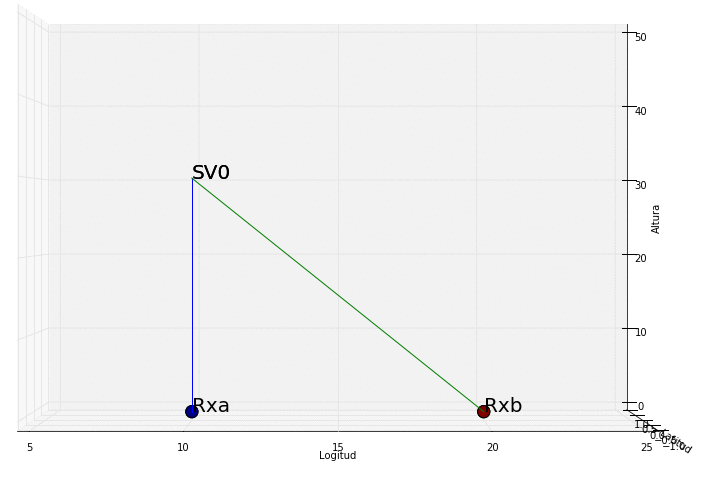
\includegraphics[scale=0.4]{Imagenes/SingleDifferencing.png}
	\caption{Diferenciamiento sencillo.}
	\label{fig:SingleDifferencing}
\end{figure}

Por términos prácticos y con el propósito de tener mayor claridad, se asume el uso del observable de medición será el pseudo-rango expresado en la ecuación \ref{eq:Ec3}. Donde el termino $\epsilon_{r}^{s}$, representa la combinación de los términos de ruido ($\eta$) y multipath ($M_{r,P}^{s}(t)$).\\ 

Los términos $d_{iono}^{s}$ y $d_{trop}^{s}$, pueden asumirse similares para ambos receptores conforme a lo expuesto en los estudios \cite{el1994effect}, \cite{blewitt1997basics}; de esta forma los observables de medición para cada receptor con respecto a un solo satélite, serían:\\

%http://tex.stackexchange.com/questions/8936/how-to-break-a-long-equation
\begin{equation}
	\begin{aligned}
		P_{A}^{s}(t) = \rho_{A}^{s}(t) +c*\tau_{A}(t) - c*\tau^{s}(t) -d_{iono}^{s} + d_{trop}^{s} + \epsilon_{A}^{s}\\
		P_{B}^{s}(t) = \rho_{B}^{s}(t) +c*\tau_{B}(t) - c*\tau^{s}(t) -d_{iono}^{s} + d_{trop}^{s} + \epsilon_{B}^{s}
	\label{eq:Ec3}
	\end{aligned}
\end{equation}\\

La operación de diferenciamiento entre los observables presentados en la ecuación \ref{eq:Ec3}, se define como $\bigtriangleup P_{AB}^{s}$:\\

\begin{equation}
	\begin{aligned}
		\bigtriangleup P_{AB}^{s} 
		& = P_{B}^{s} - P_{A}^{s}\\
		& =(\rho_{B}^{s}-\rho_{A}^{s}) + c*(\tau_{B} - \tau_{A}) + (\epsilon_{B}^{s} - \epsilon_{A}^{s})\\
		& = \bigtriangleup \rho_{AB}^{s} + c*\bigtriangleup (\tau_{AB}) + \bigtriangleup(\epsilon_{AB}^{s})
	\label{eq:Ec4}
	\end{aligned}
\end{equation}\\


%\subsubsection{
\textbf{Doble diferenciamiento.}\\

El modelo de doble diferenciamiento, también conocida como "diferenciamiento entre satélites"\cite{van2008gps} - es el diferenciamiento entre dos diferenciales sencillos según lo define, con lo que básicamente se encuentra la diferencia entre las observaciones de 2 receptores con respecto a un par satélites.\\

\begin{figure}[ht]
	\centering
	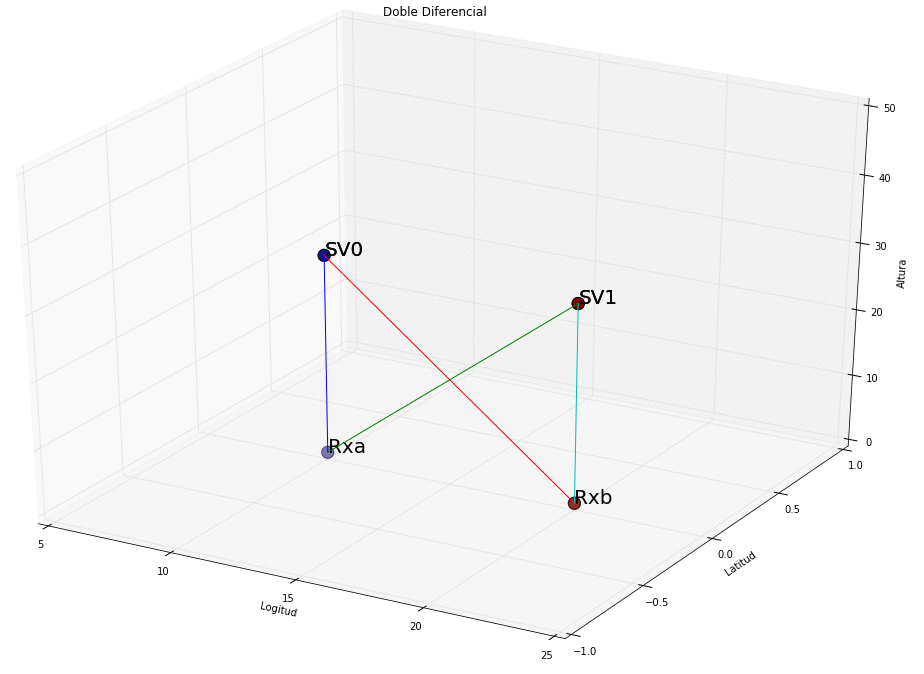
\includegraphics[scale=0.4]{Imagenes/DoubleDifferencing.png}
	\caption{Doble diferenciamiento.}
	\label{fig:DoubleDifferencing}
\end{figure}

Retomando la ecuación ~\ref{eq:Ec4}, que es el resultado entre el diferenciamiento de los observables de un receptor A y B con respecto a un satélite y considerando el escenario de la figura \textbf{\ref{fig:DoubleDifferencing}}, se tiene que:

\begin{equation}
	\begin{aligned}
		\bigtriangledown\bigtriangleup P_{AB}^{12} 
		& = \bigtriangleup P_{AB}^{2} - \bigtriangleup P_{A}^{1}\\
		& = \bigtriangleup \rho_{AB}^{12} + \bigtriangleup\epsilon_{AB}^{12}
	\label{eq:Ec5}
	\end{aligned}
\end{equation}

Donde el símbolo $\bigtriangledown$ representa la segunda operación de diferenciamiento con respecto a un segundo satélite en común entre los receptores A y B.\\

Según se expresa en la ecuación \ref{eq:Ec5}, al desarrollar la operación de doble diferenciamiento, los términos asociados con la mala sincronización en los relojes de los satélites y los receptores, son eliminados. Quedando el término $\epsilon_{r}^{s}$, quien representa la combinación de los términos de ruido ($\eta$) y multipath ($M_{r,P}^{s}(t)$).

%% Pag 36 Documento Relative Positioning

% Debido a que pueden existir tantas operaciones de doble diferenciamiento como tantos pares de receptores tengan pares de satélites en común, es probable que los resultados de la aplicación de doble diferenciamiento puedan ser una combinación lineal de sus semejantes; generando información inútil para llevar a cabo la tarea de posicionamiento.\\

% Para evitar este inconveniente la creación de un receptor y un satélite de referencia, sobre los cuales se tienen operaciones de doble diferenciamiento que arrojan resultados de observables que son linealmente independientes.\\

%Sin embargo para garantizar la selección de un receptor de referencia apropiado entre todos los disponibles, lo ideal es seleccionar aquel que tiene mayor visibilidad a satélites y a los demás receptores que lo rodean, de forma que sus semejantes se puedan beneficiar de él para realizar correcciones en sus observables; considerando que este receptor de referencia por tener mejor visibilidad de satélites, el error asociado al fenómeno de multipath se ve minimizado.\\ 

% En cuanto a la elección del satélite de referencia, el seleccionar el satélite con mayor elevación entre la lista de satélites comunes entre los receptores, de forma que este puede ser visto desde a todos ellos y además les garantiza que el efecto multipath y retraso atmosférico (ionosférico y troposférico) son reducidos.\\